%\PassOptionsToPackage{draft}{graphicx}
%\documentclass[10pt]{beamer} % aspect ratio 4:3, 128 mm by 96 mm
\documentclass[10pt,aspectratio=169]{beamer} % aspect ratio 16:9
%\graphicspath{{../../figures/}}
\graphicspath{{figs/}}
%\includeonlyframes{frame1,frame2,frame3}

%%%%%%%%%%%%%%%%%%%%%%%%%%%%%%%%%%%%%%%%%%%%%%%%%%
% Packages
%%%%%%%%%%%%%%%%%%%%%%%%%%%%%%%%%%%%%%%%%%%%%%%%%%
\usepackage{appendixnumberbeamer}
\usepackage{booktabs}
\usepackage{csvsimple} % for csv read
\usepackage[scale=2]{ccicons}
\usepackage{pgfplots}
\usepackage{xspace}
\usepackage{amsmath}
\usepackage{totcount}
\usepackage{tikz}
\usepackage{bm}
\usepackage{float}
\usepackage{eso-pic} 
\usepackage{wrapfig}
\usepackage{animate,media9,movie15}
\usepackage{subfig}

\usepackage{multimedia}
%\usepackage{FiraSans}

%\usepackage{comment}
%\usetikzlibrary{external} % speedup compilation
%\tikzexternalize % activate!
%\usetikzlibrary{shapes,arrows}  

%\usepackage{bibentry}
%\nobibliography*
\usepackage{ifthen}
\newcounter{angle}
\setcounter{angle}{0}
%\usepackage{bibentry}
%\nobibliography*
\usepackage{caption}%

\captionsetup[figure]{labelformat=empty}%
\graphicspath{{figures/}}
\usefonttheme{structurebold}
%%%%%%%%%%%%%%%%%%%%%%%%%%%%%%%%%%%%%%%%%%%%%%%%%%
% Metropolis theme custom modification file
%%%%%%%%%%%%%%%%%%%%%%%%%%%%%%%%%%%%%%%%%%%%%%%%%%
% Metropolis theme custom modification file
%%%%%%%%%%%%%%%%%%%%%%%%%%%%%%%%%%%%%%%%%%%%%%%%%%
% Metropolis theme custom colors
%%%%%%%%%%%%%%%%%%%%%%%%%%%%%%%%%%%%%%%%%%%%%%%%%%
\usetheme[progressbar=foot]{metropolis}
\useoutertheme{metropolis}
\useinnertheme{metropolis}
\usefonttheme{metropolis}
\setbeamercolor{background canvas}{bg=white}

%\usecolortheme{spruce}

\definecolor{myblue}{rgb}{0.19,0.55,0.91}
\definecolor{mediumblue}{rgb}{0,0,205}
\definecolor{darkblue}{rgb}{0,0,139}
\definecolor{Dodgerblue}{HTML}{1E90FF}
\definecolor{Navy}{HTML}{000080} % {rgb}{0,0,128}
\definecolor{Aliceblue}{HTML}{F0F8FF}
\definecolor{Lightskyblue}{HTML}{87CEFA}
\definecolor{logoblue}{RGB}{1,67,140}
\definecolor{Purple}{HTML}{911146}
\definecolor{Orange}{HTML}{CF4A30}

\setbeamercolor{progress bar}{bg=Lightskyblue}
\setbeamercolor{progress bar}{ fg=logoblue} 
\setbeamercolor{frametitle}{bg=logoblue}
\setbeamercolor{title separator}{fg=logoblue}
\setbeamercolor{block title}{bg=Lightskyblue!30,fg=black}
\setbeamercolor{block body}{bg=Lightskyblue!15,fg=black}
\setbeamercolor{alerted text}{fg=Purple}
% notes colors
\setbeamercolor{note page}{bg=white}
\setbeamercolor{note title}{bg=Lightskyblue}
%%%%%%%%%%%%%%%%%%%%%%%%%%%%%%%%%%%%%%%%%%%%%%%%%%
%  Theme modifications
%%%%%%%%%%%%%%%%%%%%%%%%%%%%%%%%%%%%%%%%%%%%%%%%%%
% modify progress bar linewidth
\makeatletter
\setlength{\metropolis@progressinheadfoot@linewidth}{2pt} 
\setlength{\metropolis@titleseparator@linewidth}{1pt}
\setlength{\metropolis@progressonsectionpage@linewidth}{1pt}

\setbeamertemplate{progress bar in section page}{
	\setlength{\metropolis@progressonsectionpage}{%
		\textwidth * \ratio{\thesection pt}{\totvalue{totalsection} pt}%
	}%
	\begin{tikzpicture}
		\fill[bg] (0,0) rectangle (\textwidth, 
		\metropolis@progressonsectionpage@linewidth);
		\fill[fg] (0,0) rectangle (\metropolis@progressonsectionpage, 
		\metropolis@progressonsectionpage@linewidth);
	\end{tikzpicture}%
}
\makeatother
\newcounter{totalsection}
\regtotcounter{totalsection}

\AtBeginDocument{%
	\pretocmd{\section}{\refstepcounter{totalsection}}{\typeout{Yes, prepending 
	was successful}}{\typeout{No, prepending was not successful}}%
}%
%%%%%%%%%%%%%%%%%%%%%%%%%%%%%%%%%%%%%%%%%%%%%%%%%%
%  Bibliography mods
%%%%%%%%%%%%%%%%%%%%%%%%%%%%%%%%%%%%%%%%%%%%%%%%%%
\setbeamertemplate{bibliography item}{\insertbiblabel} %% Remove book symbol 
%%from references and add number in square brackets
% kill the abominable icon (without number)
%\setbeamertemplate{bibliography item}{}
%\makeatletter
%\renewcommand\@biblabel[1]{#1.} % number only
%\makeatother
% remove line breaks in bibliography
\setbeamertemplate{bibliography entry title}{}
\setbeamertemplate{bibliography entry location}{}
%%%%%%%%%%%%%%%%%%%%%%%%%%%%%%%%%%%%%%%%%%%%%%%%%%
%  Bibliography custom commands
%%%%%%%%%%%%%%%%%%%%%%%%%%%%%%%%%%%%%%%%%%%%%%%%%%
\newcommand{\bibliotitlestyle}[1]{\textbf{#1}\par}

\newif\ifinbiblio
\newcounter{bibkey}
\newenvironment{biblio}[2][long]{%
	%\setbeamertemplate{bibliography item}{\insertbiblabel}
	\setbeamertemplate{bibliography item}{}% without numbers
	\setbeamerfont{bibliography item}{size=\footnotesize}
	\setbeamerfont{bibliography entry author}{size=\footnotesize}
	\setbeamerfont{bibliography entry title}{size=\footnotesize}
	\setbeamerfont{bibliography entry location}{size=\footnotesize}
	\setbeamerfont{bibliography entry note}{size=\footnotesize}
	\ifx!#2!\else%
	\bibliotitlestyle{#2}%
	\fi%
	\begin{thebibliography}{}%
		\inbibliotrue%
		\setbeamertemplate{bibliography entry title}[#1]%
	}{%
		\inbibliofalse%
		\setbeamertemplate{bibliography item}{}%
	\end{thebibliography}%
}

\newcommand{\biblioref}[5][short]{
	\setbeamertemplate{bibliography entry title}[#1]
	\stepcounter{bibkey}%
	\ifinbiblio%
	\bibitem{\thebibkey}%
	#2
	\newblock #4
	\ifx!#5!\else\newblock {\em #5}, #3 \fi%
	\else%
	\begin{biblio}{}
		\bibitem{\thebibkey}
		#2
		\newblock #4
		\ifx!#5!\else\newblock {\em #5}, #3\fi
	\end{biblio}
	\fi
}
%
%\newbibmacro*{hypercite}{%
%	\renewcommand{\@makefntext}[1]{\noindent\normalfont##1}%
%	\footnotetext{%
%		\blxmkbibnote{foot}{%
%			\printtext[labelnumberwidth]{%
%				\printfield{prefixnumber}%
%				\printfield{labelnumber}}%
%			\addspace
%			\fullcite{\thefield{entrykey}}}}}
%
%\DeclareCiteCommand{\hypercite}%
%{\usebibmacro{cite:init}}
%{\usebibmacro{hypercite}}
%{}
%{\usebibmacro{cite:dump}}
%
%% Redefine the \footfullcite command to use the reference number
%\renewcommand{\footfullcite}[1]{\cite{#1}\hypercite{#1}}
%\usefonttheme[onlymath]{Serif}  % It should be uncommented if Fira fonts in 
%%math does not work

%%%%%%%%%%%%%%%%%%%%%%%%%%%%%%%%%%%%%%%%%%%%%%%%%%
% Custom commands
%%%%%%%%%%%%%%%%%%%%%%%%%%%%%%%%%%%%%%%%%%%%%%%%%%
% matrix command 
\newcommand{\matr}[1]{\mathbf{#1}} % bold upright (Elsevier, Springer)
%\newcommand{\matr}[1]{#1}          % pure math version
%\newcommand{\matr}[1]{\bm{#1}}     % ISO complying version
% vector command 
\newcommand{\vect}[1]{\mathbf{#1}} % bold upright (Elsevier, Springer)
% bold symbol
\newcommand{\bs}[1]{\boldsymbol{#1}}
% derivative upright command
\DeclareRobustCommand*{\drv}{\mathop{}\!\mathrm{d}}
\newcommand{\ud}{\mathrm{d}}
% 
\newcommand{\themename}{\textbf{\textsc{metropolis}}\xspace}


%%%%%%%%%%%%%%%%%%%%%%%%%%%%%%%%%%%%%%%%%%%%%%%%%%
%  Title page options
%%%%%%%%%%%%%%%%%%%%%%%%%%%%%%%%%%%%%%%%%%%%%%%%%%
% \date{\today}
\date{}
%%%%%%%%%%%%%%%%%%%%%%%%%%%%%%%%%%%%%%%%%%%%%%%%%%
% option 1
%%%%%%%%%%%%%%%%%%%%%%%%%%%%%%%%%%%%%%%%%%%%%%%%%%%
\title{Delamination identification using global convolution networks}
\subtitle{European Workshop on Structural Health Monitoring \\ EWSHM 2022, Palermo-Italy}

\author{\textbf{Abdalraheem Ijjeh\\Supervisor: Prof. Paweł Kudela}}
% logo align to Institute 
\institute{Institute of Fluid Flow Machinery \\ 
	Polish Academy of Sciences \\ 
	\vspace{-1.5cm}
	\flushright 
	\includegraphics[width=6cm]{imp_logo.png}}
%%%%%%%%%%%%%%%%%%%%%%%%%%%%%%%%%%%%%%%%%%%%%%%%%%
% option 2 - authors in one line
%%%%%%%%%%%%%%%%%%%%%%%%%%%%%%%%%%%%%%%%%%%%%%%%%%
%	\title{My fancy title}
%	\subtitle{Lamb-opt}
%	\author{\textbf{Paweł Kudela}\textsuperscript{2}, Maciej 
%	Radzieński\textsuperscript{2}, Wiesław Ostachowicz\textsuperscript{2}, 
%	Zhibo Yang\textsuperscript{1} }
%	 logo align to Institute 
%	\institute{\textsuperscript{1}Xi'an Jiaotong University \\ 
%	\textsuperscript{2}Institute of Fluid Flow Machinery\\ \hspace*{1pt} Polish 
%	Academy of Sciences \\ \vspace{-1.5cm}\flushright 
%	
%\includegraphics[width=4cm]{//odroid-sensors/sensors/MISD_shared/logo/logo_eng_40mm.eps}}
%%%%%%%%%%%%%%%%%%%%%%%%%%%%%%%%%%%%%%%%%%%%%%%%%%%
% option 3 - multilogo vertical
%%%%%%%%%%%%%%%%%%%%%%%%%%%%%%%%%%%%%%%%%%%%%%%%%%
%%\title{My fancy title}
%%\subtitle{Lamb-opt}
%%	\author{\textbf{Paweł Kudela}\inst{1}, Maciej Radzieński\inst{1}, Wiesław Ostachowicz\inst{1}, Zhibo Yang\inst{2} }
%%	 logo under Institute 
%%	\institute%
%%	{ 
%%		\inst{1}%
%%		Institute of Fluid Flow Machinery\\ \hspace*{1pt} Polish Academy of Sciences \\ \includegraphics[height=0.85cm]{//odroid-sensors/sensors/MISD_shared/logo/logo_eng_40mm.eps} \\
%%		\and
%%		\inst{2}%
%%	    Xi'an Jiaotong University \\ \includegraphics[height=0.85cm]{//odroid-sensors/sensors/MISD_shared/logo/logo_box.eps}
%%    }
% end od option 3
%%%%%%%%%%%%%%%%%%%%%%%%%%%%%%%%%%%%%%%%%%%%%%%%%%
%% option 4 - 3 Institutes and logos horizontal centered
%%%%%%%%%%%%%%%%%%%%%%%%%%%%%%%%%%%%%%%%%%%%%%%%%%
%\title{My fancy title}
%\subtitle{Lamb-opt }
%\author{\textbf{Paweł Kudela}\textsuperscript{1}, Maciej Radzieński\textsuperscript{1}, Marco Miniaci\textsuperscript{2}, Zhibo Yang\textsuperscript{3} }
%
%\institute{ 
%\begin{columns}[T,onlytextwidth]
%	\column{0.39\textwidth}
%	\begin{center}
%		\textsuperscript{1}Institute of Fluid Flow Machinery\\ \hspace*{3pt}Polish Academy of Sciences
%	\end{center}
%	\column{0.3\textwidth}
%	\begin{center}
%		\textsuperscript{2}Zurich University
%	\end{center}
%	\column{0.3\textwidth}
%	\begin{center}
%		\textsuperscript{3}Xi'an Jiaotong University
%	\end{center}
%\end{columns}
%\vspace{6pt}
%% logos 
%\begin{columns}[b,onlytextwidth]
%	\column{0.39\textwidth}
%		\centering 
%		\includegraphics[scale=0.9,height=0.85cm,keepaspectratio]{//odroid-sensors/sensors/MISD_shared/logo/logo_eng_40mm.eps}
%	\column{0.3\textwidth}
%		\centering 
%		\includegraphics[scale=0.9,height=0.85cm,keepaspectratio]{//odroid-sensors/sensors/MISD_shared/logo/logo_box.eps}
%	\column{0.3\textwidth}
%		\centering 
%		\includegraphics[scale=0.9,height=0.85cm,keepaspectratio]{//odroid-sensors/sensors/MISD_shared/logo/logo_box2.eps}
%\end{columns}
%}
%\makeatletter
%\setbeamertemplate{title page}{
%	\begin{minipage}[b][\paperheight]{\textwidth}
%		\centering  % <-- Center here
%		\ifx\inserttitlegraphic\@empty\else\usebeamertemplate*{title graphic}\fi
%		\vfill%
%		\ifx\inserttitle\@empty\else\usebeamertemplate*{title}\fi
%		\ifx\insertsubtitle\@empty\else\usebeamertemplate*{subtitle}\fi
%		\usebeamertemplate*{title separator}
%		\ifx\beamer@shortauthor\@empty\else\usebeamertemplate*{author}\fi
%		\ifx\insertdate\@empty\else\usebeamertemplate*{date}\fi
%		\ifx\insertinstitute\@empty\else\usebeamertemplate*{institute}\fi
%		\vfill
%		\vspace*{1mm}
%	\end{minipage}
%}
%
%\setbeamertemplate{title}{
%	%  \raggedright%  % <-- Comment here
%	\linespread{1.0}%
%	\inserttitle%
%	\par%
%	\vspace*{0.5em}
%}
%\setbeamertemplate{subtitle}{
%	%  \raggedright%  % <-- Comment here
%	\insertsubtitle%
%	\par%
%	\vspace*{0.5em}
%}
%\makeatother
% end of option 4
%%%%%%%%%%%%%%%%%%%%%%%%%%%%%%%%%%%%%%%%%%%%%%%%%%
% option 5 - 2 Institutes and logos horizontal centered
%%%%%%%%%%%%%%%%%%%%%%%%%%%%%%%%%%%%%%%%%%%%%%%%%%
%\title{My fancy title}
%\subtitle{Lamb-opt }
%\author{\textbf{Paweł Kudela}\textsuperscript{1}, Maciej Radzieński\textsuperscript{1}, Marco Miniaci\textsuperscript{2}}
%
%\institute{ 
%	\begin{columns}[T,onlytextwidth]
%		\column{0.5\textwidth}
%			\centering
%			\textsuperscript{1}Institute of Fluid Flow Machinery\\ \hspace*{3pt}Polish Academy of Sciences
%		\column{0.5\textwidth}
%			\centering
%			\textsuperscript{2}Zurich University
%	\end{columns}
%	\vspace{6pt}
%	% logos 
%	\begin{columns}[b,onlytextwidth]
%		\column{0.5\textwidth}
%		\centering 
%		\includegraphics[scale=0.9,height=0.85cm,keepaspectratio]{//odroid-sensors/sensors/MISD_shared/logo/logo_eng_40mm.eps}
%		\column{0.5\textwidth}
%		\centering 
%		\includegraphics[scale=0.9,height=0.85cm,keepaspectratio]{//odroid-sensors/sensors/MISD_shared/logo/logo_box.eps}
%	\end{columns}
%}
%\makeatletter
%\setbeamertemplate{title page}{
%	\begin{minipage}[b][\paperheight]{\textwidth}
%		\centering  % <-- Center here
%		\ifx\inserttitlegraphic\@empty\else\usebeamertemplate*{title graphic}\fi
%		\vfill%
%		\ifx\inserttitle\@empty\else\usebeamertemplate*{title}\fi
%		\ifx\insertsubtitle\@empty\else\usebeamertemplate*{subtitle}\fi
%		\usebeamertemplate*{title separator}
%		\ifx\beamer@shortauthor\@empty\else\usebeamertemplate*{author}\fi
%		\ifx\insertdate\@empty\else\usebeamertemplate*{date}\fi
%		\ifx\insertinstitute\@empty\else\usebeamertemplate*{institute}\fi
%		\vfill
%		\vspace*{1mm}
%	\end{minipage}
%}
%
%\setbeamertemplate{title}{
%	%  \raggedright%  % <-- Comment here
%	\linespread{1.0}%
%	\inserttitle%
%	\par%
%	\vspace*{0.5em}
%}
%\setbeamertemplate{subtitle}{
%	%  \raggedright%  % <-- Comment here
%	\insertsubtitle%
%	\par%
%	\vspace*{0.5em}
%}
%\makeatother
% end of option 5
%
%%%%%%%%%%%%%%%%%%%%%%%%%%%%%%%%%%%%%%%%%%%%%%%%%%
%  End of title page options
%%%%%%%%%%%%%%%%%%%%%%%%%%%%%%%%%%%%%%%%%%%%%%%%%%
% logo option - alternative manual insertion by modification of coordinates in \put()
%\titlegraphic{%
%	%\vspace{\logoadheight}
%	\begin{picture}(0,0)
%	\put(305,-185){\makebox(0,0)[rb]{\includegraphics[width=4cm]{//odroid-sensors/sensors/MISD_shared/logo/logo_eng_40mm.eps}}}
%	\end{picture}}
%
%%%%%%%%%%%%%%%%%%%%%%%%%%%%%%%%%%%%%%%%%%%%%%%%%%
%\tikzexternalize % activate!
%%%%%%%%%%%%%%%%%%%%%%%%%%%%%%%%%%%%%%%%%%%%%%%%%%
\begin{document}
	

%%%%%%%%%%%%%%%%%%%%%%%%%%%%%%%%%%%%%%%%%%%%%%%%%%
\maketitle
\note{
	Welcome and thank you for joining me here at this remote presentation event. At the beginning I want to introduce my self, my name is Abdalrheem Ijjeh, a PhD student at the Institute of Fluid flow machinery, Polish academy of sciences, supervised by professor Pawel Kudela. Today I am going to briefly present my PhD project entitled by  Feasibility studies of artificial intelligence-driven diagnostics}
%%%%%%%%%%%%%%%%%%%%%%%%%%%%%%%%%%%%%%%%%%%%%%%%%%
% SLIDES
%%%%%%%%%%%%%%%%%%%%%%%%%%%%%%%%%%%%%%%%%%%%%%%%%%
\begin{frame}[label=frame1]{Outlines}
  	\setbeamertemplate{section in toc}[sections numbered]
	\tableofcontents
\end{frame}
\note{
	The presentation will be as follow: 
	In the first section, I am going to introduce and define composite materials, then I will talk briefly about defects in composite materials, and the conventional approach of damage detection in composite materials. \\
	In the second section, I will briefly introduce Artificial intelligence, machine learning and deep learning approaches.\\
	In the third section, the objectives of the project will be presented. \\
	Then I will talk about the Dataset generation in the fourth section. \\
	Finally, in the last section, I am going to talk about deep learning techniques for delamination identification.}
%%%%%%%%%%%%%%%%%%%%%%%%%%%%%%%%%%%%%%%%%%%%%%%%%%
\section{Composite laminates}
%%%%%%%%%%%%%%%%%%%%%%%%%%%%%%%%%%%%%%%%%%%%%%%%%%
\subsection{Delamination in composite laminates}
\begin{frame}{Defects of composite laminates}
	\small		
	Composite laminates can have different types of damage such as: \\
	\textbf{Cracks, fibre breakage, debonding, and delamination.} \\ 
	\begin{minipage}[c]{.40\textwidth}	
		
		\begin{itemize}
			\footnotesize	
			\item Delamination is a critical failure mechanism in laminated fibre-reinforced polymer matrix composites.
			\item Delamination is one of the most hazardous forms of the defects. 
			It leads to very catastrophic failures if not detected at early stages.
		\end{itemize}
	
	\end{minipage}
	\hfill
	\begin{minipage}[c]{0.50\textwidth}
%		\begin{figure}[h!]
		\subfloat{\includegraphics[width=.95\textwidth]{damage_composites.png}}
%		\end{figure}
		\tiny
			(source: https://industrialndt.com/ultrasonic-testing-for-fiber-glass-reinforced-plastic/)
	\end{minipage}
\end{frame}
\note{
	Generally, impact damage in composite materials is caused by various impact events that result from the lack of reinforcement in the out-of-plane direction.
	Causing: 
	Matrix cracks, 
	Fibre breakage, 
	Debonding (occurs when an adhesive stops adhering to an adherend) 
	And delamination, as shown in the figure, which can alter the compression strength of composite laminate and gradually affect the composite to encounter failure by buckling.
	Among these defects in composites, delamination is considered one of the most hazardous types of defects. 
	That is because delamination can seriously decrease the performance of the composite.
	Therefore, delamination detection in the early stages can help to avoid structural collapses.
	}
%%%%%%%%%%%%%%%%%%%%%%%%%%%%%%%%%%%%%%%%%%%%%%%%%%
\subsection{Damage detection in composite laminates}
%%%%%%%%%%%%%%%%%%%%%%%%%%%%%%%%%%%%%%%%%%%%%%%%%%
\begin{frame}{Conventional approaches}
	Conventional structural damage detection methods involve two processes:
	\begin{itemize}
		\item \textbf{Feature extraction}
		\item \textbf{Feature classification}
	\end{itemize}
	\subfloat{\includegraphics[width=.95\textwidth]{conventional_ML.png}}
		Drawbacks of Conventional methods:
	\begin{itemize}
		\item Requires a great amount of human labor and computational effort.
		\item Demands a high amount of experience of the practitioner.
		\item Inefficient with big data which requires a complex computation of damage features.  
	\end{itemize}
\end{frame}
\note{
	In conventional damage detection methods, to detect the damage, first, we must analyse the response of structure obtained by sensors such as (PZTs) that can sense for example the generated guided waves (e.g. Lamb waves). 
	Then, we need to extract the features of response  (which requires large computational effort). 
	Then we can attempt to classify these features, which are sensitive to minor damage and that can be distinguished from the response to natural and environmental changes (baseline).
	}
%%%%%%%%%%%%%%%%%%%%%%%%%%%%%%%%%%%%%%%%%%%%%%%%%%
\note{
	Conventional methods of damage detection focus on patterns
	extraction from registered measurements and accordingly make decisions based on these patterns. 
	Moreover, conventional methods for pattern recognition require feature selection and classification (handcrafted features). 
	These conventional methods can perform efficient damage detection. However, these methods depend on selected features from their scope of measurement. 
	Accordingly, introducing new patterns will cause them to fail in detecting the damage.
	Furthermore, these methods could fail in detecting damage when dealing with big data requiring a complex computation of damage features.
}
\setcounter{subfigure}{0}
\section{Deep learning based approach}
%%%%%%%%%%%%%%%%%%%%%%%%%%%%%%%%%%%%%%%%%%%%%%%%%%
%%%%%%%%%%%%%%%%%%%%%%%%%%%%%%%%%%%%%%%%%%%%%%%%%%
%\subsection{Introduction to deep learning}
%%%%%%%%%%%%%%%%%%%%%%%%%%%%%%%%%%%%%%%%%%%%%%%%%%
%\begin{frame}{What is deep learning?}
%	\begin{figure}
%		\centering
%		\includegraphics[width=0.85\textwidth]{AI_vs_ML_vs_Deep_Learning.png}
%	\end{figure}
%	\tiny
%	(source: https://www.ingeniovirtual.com/)
%\end{frame}

%\setcounter{subfigure}{0}
%%%%%%%%%%%%%%%%%%%%%%%%%%%%%%%%%%%%%%%%%%%%%%%%%%%
%\begin{frame}{Deep learning, why now?}
%	\begin{minipage}[c]{0.4\textwidth}
%		AI technologies are in accelerating growth due to:
%		\begin{itemize}
%			\item Exponential development in computer hardware industries
%			 (e.g. CPUs, GPUs, FPGAs, TPUs and ASICs)
%			\item Era of Big data, 	
%		\end{itemize}
%	\end{minipage}
%	\begin{minipage}[c]{0.55\textwidth}
%		\begin{figure}
%			\centering
%			\subfloat{\animategraphics[autoplay,loop,width=.9\textwidth]{10}{figures/gif_figs/gpu/gpu_-}{0}{34}}			
%		\end{figure}
%	\tiny
%	(source: https://www.techbooky.com/)	
%	\end{minipage}
%	
%\end{frame}
%%%%%%%%%%%%%%%%%%%%%%%%%%%%%%%%%%%%%%%%%%%%%%%%%%
%\setcounter{subfigure}{0}
%%%%%%%%%%%%%%%%%%%%%%%%%%%%%%%%%%%%%%%%%%%%%%%%%%%
%\begin{frame}{Common learning strategies}
%	\centering			
%	\begin{figure}
%		\includegraphics[width=0.9\textwidth]{learning.png}
%	\end{figure}
%	\tiny
%	(source: https://www.aitude.com/supervised-vs-unsupervised-vs-reinforcement/)
%\end{frame}
%\setcounter{subfigure}{0}
%\begin{frame}{Artificial neuron}	
%	\begin{minipage}[c]{0.40\textwidth}
%		\begin{itemize}
%			\item 	Neuron is responsible for acting as a gate (previous-to-next) layers with a nonlinear operation.	
%		\end{itemize}
%		\begin{equation}
%			y = f(\sum_{i=0}^{n}w_{i}x_i+ b)
%		\end{equation}
%	\end{minipage}
%	\begin{minipage}[c]{0.55\textwidth}
%		\begin{figure}
%			\centering
%			\subfloat[Biological neuron]{\includegraphics[width=.75\textwidth]{real_neuron.png}} \\
%			\subfloat[Artificial neuron]{\includegraphics[width=0.65\textwidth]{neuron.png}} 
%		\end{figure}
%	\end{minipage}
%	
%\end{frame}

%\setcounter{subfigure}{0}
%\begin{frame}{Artificial neural networks}
%	\begin{minipage}[c]{0.4\textwidth}
%		Artificial neural network (ANN) can be created by cascading n-layers of “neurons”. 
%		\begin{itemize}
%			\item Input layer.
%			\item Hidden layer(s).
%			\item Output layer.	
%		\end{itemize}
%	\end{minipage}
%	\hfill
%	\begin{minipage}[c]{0.55\textwidth}
%		\centering
%		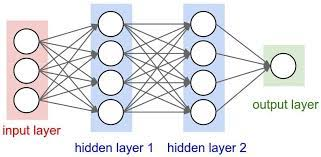
\includegraphics[width=0.95\textwidth]{ann.png}
%	\end{minipage}	
%\end{frame}

%
%\setcounter{subfigure}{0}
%\begin{frame}{Convolutional neural networks}
%	\begin{minipage}[c]{0.35\textwidth}
%		\textbf{Convolution operation}\\
%		\subfloat{\animategraphics[autoplay,loop, controls,width=4cm]{1}{figures/gif_figs/conv_op/conv_op-}{0}{8}}
%	\end{minipage}
%	\begin{minipage}[0]{0.6\textwidth}
%		\subfloat{\includegraphics[[width=0.95\textwidth]{cnn.png}}
%	\end{minipage}
%	\tiny
%	(source: https://github.com/tbozinis/simple-convolution)
%\end{frame}
%\setcounter{subfigure}{0}
%%%%%%%%%%%%%%%%%%%%%%%%%%%%%%%%%%%%%%%%%%%%%%%%%%%
%\begin{frame}{Training process}
%	
%	\begin{minipage}[ct]{0.4\textwidth}
%			\begin{itemize}
%				\footnotesize
%				\item Feed-forward pass (initial predictions are done).
%				\item Calculating the loss between the prediction and actual  values via optimization process e.g. (Gradient descent).
%				\item Updating all learnable parameters using backpropagation technique.				
%				\begin{equation}
%					w_{jk}\leftarrow w_{jk}-\alpha \frac{\partial J}{\partial w_{jk}}					
%				\end{equation}
%				\begin{equation}										
%					b_{jk}\leftarrow b_{jk}-\alpha \frac{\partial J}{\partial b_{jk}}
%				\end{equation}
%			\end{itemize}
%		
%	\end{minipage}
%\hfill
%	\begin{minipage}[c]{0.55\textwidth}
%		\begin{figure}
%			\centering
%			\subfloat{\animategraphics[autoplay,loop, controls,width=6cm]{2}{figures/gif_figs/sgd/SGD.gif-}{0}{10}}
%		\end{figure}
%	\tiny
%	(source: https://suniljangirblog.files.wordpress.com/2018/12/1-1.gif?w=379
%	)
%	\end{minipage}
%
%\end{frame}
\begin{frame}{Why deep learning?}
	\centering
	\textbf{End-to-end approach} 
	\par\medskip
	\subfloat{\includegraphics[width=.95\textwidth]{DL_approach.png}}
\end{frame}
%%%%%%%%%%%%%%%%%%%%%%%%%%%%%%%%%%%%%%%%%%%%%%%%%%%%%%%%%%%%%%%%%%%%%%%%%%%%%%%%
\subsection{Computer vision}
\setcounter{subfigure}{0}
\begin{frame}{What is computer vision?}
	\begin{minipage}[c]{0.30\textwidth}
		Computer vision is a field of AI that enables computers and systems to derive meaningful information from digital images, videos and other visual inputs. 
	\end{minipage}
	\hfill
	\begin{minipage}[c]{0.65\textwidth}
		\begin{figure}
			\centering
			\includegraphics[width=1\textwidth]{computer_vision_tasks.png}
		\end{figure}
	\end{minipage}
\end{frame}
%%%%%%%%%%%%%%%%%%%%%%%%%%%%%%%%%%%%%%%%%%%%%%%%%%
\subsection{Synthetic Dataset generation}
\setcounter{subfigure}{0}
%%%%%%%%%%%%%%%%%%%%%%%%%%%%%%%%%%%%%%%%%%%%%%%%%%
\begin{frame}{Dataset description}
	\centering
	\begin{minipage}[c]{0.35\textwidth}
		\begin{itemize}
			\justifying
			\item 475 cases.
			\item Delamination has a different shape, size and location for each case.
			\item CFRP is made of 8-layers.
			\item Delamination was modelled between the 3rd and 4th layer.			
		\end{itemize}
	\end{minipage}
	\hfill
	\begin{minipage}[c]{0.6\textwidth}
		\begin{figure}
			\centering			
			\subfloat[Delamination orientation \label{fig:1}]{\includegraphics[width=0.52\textwidth]{figure1.png}}\qquad
			\subfloat[all cases overlapped \label{fig:2}]{\includegraphics[width=0.35\textwidth]{figure_overlap.png}}
		\end{figure}
	\end{minipage}
\end{frame}

\setcounter{subfigure}{0}
\begin{frame}{Training Sample case}
	\begin{figure}
		\centering		
		\subfloat[Full wavefield \(s(x,y,t_k\)) \label{fig:3}]{\animategraphics[autoplay,loop, controls,width=4cm]{16}{figures/gif_figs/7_output/flat_shell_Vz_7_500x500bottom-}{1}{512}}\qquad
		\subfloat[RMS \(\hat{s}(x,y)\) \label{fig:4}]{\includegraphics[width=4cm]{RMS_flat_shell_Vz_7_500x500bottom.png}}\qquad
		\subfloat[Ground truth (label) \label{fig:5}]{\includegraphics[width=4cm]{m1_rand_single_delam_7.png}}
	\end{figure}
The RMS is defined as:
%%%%%%%%%%%%%%%
\begin{equation}
	\hat{s}(x,y) = \sqrt{\frac{1}{N}\sum_{k-1}^{N}s(x,y,t_k)^2}, 
	\label{eqn:rms} 
\end{equation}
\end{frame}


\subsection{Global Convolution Networks}
\setcounter{subfigure}{0}
\begin{frame}{Image semantic segmentation}
	\begin{minipage}[l]{0.35\textwidth}
		\textbf{One-to-one \\(RMS based approach)}
	\end{minipage}
	\begin{minipage}[l]{0.6\textwidth}
		\begin{figure}
			\centering
			\subfloat[Single input]{\includegraphics[width=.45\textwidth]{RMS_flat_shell_Vz_381_500x500bottom.png}}\qquad
			\subfloat[Single output]{\includegraphics[width=.45\textwidth]{GCN_381.png}}\qquad
		\end{figure}
	\end{minipage}	
\end{frame}


%%%%%%%%%%%%%%%%%%%%%%%%%%%%%%%%%%%%%%%%%%%%%%%%%%
\setcounter{subfigure}{0}
\begin{frame}{Global Convolution Network (GCN)}
	\begin{minipage}[ht]{0.5\textwidth}
		\begin{figure}
			\includegraphics[width=.9\textwidth]{figure8.png} 
			\caption{GCN architecture.}
		\end{figure}
	
		\end{minipage}
		\begin{minipage}[c]{0.45\textwidth}
			\begin{figure}[c]
				\centering
				\includegraphics[width=.9\textwidth]{figure9.png}
				\caption{(a) Res-block, (b) GCN block, (c) BR.}
			\end{figure}
	\end{minipage}
\end{frame}

\subsection{Numerical test cases}
\begin{frame}{Data-flow \& Intermediate outputs of layers}
	
	\begin{minipage}[c]{0.32\textwidth}
		\begin{figure}[c]
			\centering
			\animategraphics[controls,width=.9\textwidth]{2}{figures/gif_figs/397/intermediate_output-}{0}{82}
			\caption{\(1^{st}\) numerical case.}
		\end{figure}
	\end{minipage}
	\hfill
	\begin{minipage}[c]{0.32\textwidth}
		\begin{figure}[c]
			\centering
			\animategraphics[controls,width=.9\textwidth]{2}{figures/gif_figs/438/intermediate_output-}{0}{82}
			\caption{\(2^{nd}\) numerical case.}
		\end{figure}
	\end{minipage}
	\hfill
	\begin{minipage}[c]{0.32\textwidth}
		\begin{figure}[c]
			\centering
			\animategraphics[controls,width=.9\textwidth]{2}{figures/gif_figs/456/intermediate_output-}{0}{82}
			\caption{\(3^{rd}\) numerical case.}
		\end{figure}
	\end{minipage}
\end{frame}


\subsection{Experimental case}
\setcounter{subfigure}{0}
\begin{frame}{Experimental setup}
	\begin{minipage}[t]{0.55\textwidth}
		\begin{figure}
			\centering
			\includegraphics[width=.9\textwidth]{wibrometr-laserowy-1d_small-description.png}
		\end{figure}
	\end{minipage}
	\begin{minipage}[t]{0.4\textwidth}
		\begin{enumerate}
			\item Waveform generator
			\item Power amplifier	
			\item Specimen
			\item SLDV head
			\item DAQ
		\end{enumerate}
	\end{minipage}
\end{frame}

\begin{frame}{Experimental results}
	\centering
	\begin{figure}
		\subfloat[ERMS \& label]{\includegraphics[width=.4\textwidth]{ERMS_with_label.png}}
		\hfill
		\subfloat[IoU\(=0.723\)]{\includegraphics[width=.4\textwidth]{Fig_GCN_7.png}}\qquad
	\end{figure}
\end{frame}
\note{		
	\begin{itemize}
		\item CFRP with Teflon insert as artificial delamination.
		\item Applied a frequency of 50 kHz to excite a signal in a transducer placed at the centre of the plate.
		\item  The measurements were performed by Polytec PSV-400 SLDV on a bottom surface of the plate of dimensions 500 by 500 mm. 
		\item The measurements were performed by Polytec PSV-400 SLDV on a bottom surface of the plate of dimensions 500 by 500 mm. 
		\item The measurement grid spacing was 1 mm and sampling frequency 512 kHz. The measured full wavefield was further processed by an energy compensated RMS takes into account wave attenuation. The results of such operation are shown in (a).
\end{itemize}}
%%%%%%%%%%%%%%%%%%%%%%%%%%%%%%%%%%%%%%%%%%%%%%%%%%
{\setbeamercolor{palette primary}{fg=blue, bg=white}
\begin{frame}[standout]
  Thank you for your listening!\\ \vspace{12pt}
  Questions?\\ \vspace{12pt}
  \url{aijjeh@imp.gda.pl}
\end{frame}
}
\note{Than you for listening, and I am  }
%%%%%%%%%%%%%%%%%%%%%%%%%%%%%%%%%%%%%%%%%%%%%%%%%%
% END OF SLIDES
%%%%%%%%%%%%%%%%%%%%%%%%%%%%%%%%%%%%%%%%%%%%%%%%%%
\end{document}